\section{Pruning}

\begin{figure}[htbp]
    \centering
    \centerline{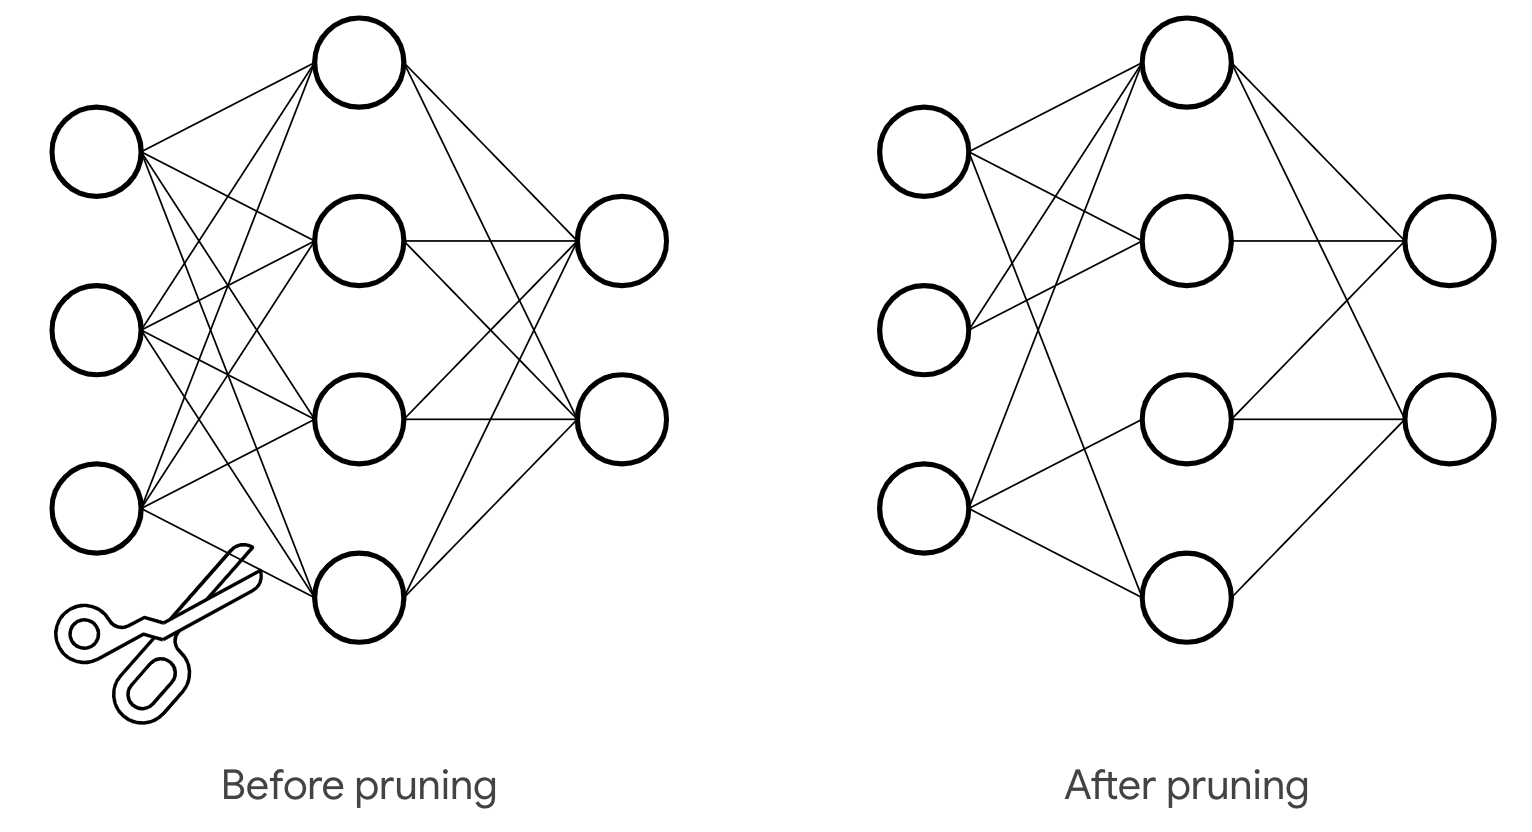
\includegraphics[width=0.8\linewidth]{images/pruning.png}}
    \caption{Pruning diagram \cite{TensorFlowModelOptimization}}
    \label{fig:pruning_diagram}
\end{figure}

Pruning is a neural network optimization technique that involves removing unnecessary parameters from a model to reduce its size, improve its computational efficiency, and potentially improve its performance in generalization. As shown in figure \ref{fig:pruning_diagram}, it involves identifying and removing the least important connections or neurons from the network and can be performed in different ways, including weight pruning, unit pruning, and filter pruning.

Filter pruning is a technique used to identify and remove the convolutional filters that contribute the least to a neural network's overall performance. The method identifies filters that produce low feature maps and remove them to reduce the overall size of the model. One particular study proposed a filter pruning technique that utilizes the L1-norm of the filters as a criterion for pruning. The method involves setting the weights of the filters to zero and then removing the filters with the smallest L1-norms. The pruning is done iteratively until the desired level of sparsity is achieved. The study showed that their pruning method can lead to significant compression of ConvNets without significant loss in accuracy \cite{liPruningFiltersEfficient2017}.

Pruning can be applied to various parts of the network, including the input layer, the hidden layers, and the output layer. In YOLOv3, for example, pruning can be applied to the detection "neck" and "head" parts of the network, which are responsible for feature extraction and object detection, respectively. The results of filter pruning to the models developed are shown in table \ref{tab:modelparaprunes}.

In the detection "neck" of YOLOv3, which consists of several convolutional layers, pruning can be applied to individual filters or channels to reduce the number of computations required for feature extraction. In the detection "head" part of YOLOv3, which consists of several fully connected layers, pruning can be applied to individual weights or neurons to reduce the size and complexity of the network.